\documentclass[11pt,aspectratio=169]{beamer}
\usetheme{Boadilla}
\usecolortheme{beaver}
\usepackage[utf8]{inputenc}
\usepackage[spanish,mexico]{babel}
\usepackage{amsmath}
\usepackage{amsfonts}
\usepackage{amssymb}
\usepackage{graphicx}
\usepackage{booktabs}
\usepackage{listings}
\usepackage{multicol}
\usepackage{multirow}
\usepackage{algorithm,algorithmic}
\usepackage{tikz}
\author{Héctor Selley}
\title{Redes neuronales}
\providecommand{\tightlist}{%
  \setlength{\itemsep}{0pt}\setlength{\parskip}{0pt}}
%\setbeamercovered{transparent} 
%\setbeamertemplate{navigation symbols}{} 
%\logo{} 
\institute{Universidad Anáhuac México} 
\date{\today} 
%\subject{} 
\begin{document}

\AtBeginSection[] % Do nothing for \section*
{
\begin{frame}<beamer>
\frametitle{Contenido}
\tableofcontents[currentsection]
\end{frame}
}

\begin{frame}
	\titlepage
\end{frame}

%\begin{frame}
%	\tableofcontents
%\end{frame}

\section{¿Qué son las Redes Neuronales?}
\begin{frame}{¿Qué son las Redes Neuronales?}
	\begin{itemize}
		\item Las redes neuronales son modelos computacionales inspirados en el funcionamiento del cerebro humano. \pause
		\item Se componen de unidades de procesamiento llamadas neuronas artificiales o nodos, que se organizan en 
			capas y se conectan entre sí mediante conexiones ponderadas.\pause
		\item Las redes neuronales tratan de imitan el funcionamiento de las redes neuronales de los organismos vivos:
			 un conjunto de neuronas conectadas entre sí y que trabajan en conjunto, sin que haya una tarea concreta para cada una.\pause
		\item Con la experiencia, las neuronas van creando y reforzando ciertas conexiones para \textit{aprender} algo que se queda fijo en el tejido.
	\end{itemize}
\end{frame}

\begin{frame}{¿Qué son las Redes Neuronales?}
	\begin{itemize}
		\item Se basan en una idea sencilla: dados unos parámetros hay una forma de combinarlos para predecir un cierto resultado.\pause
		\item Las redes neuronales son un modelo para encontrar esa combinación de parámetros y aplicarla al mismo tiempo. \pause 
		\item Esto es, encontrar la combinación que mejor se ajusta es \textit{entrenar} la red neuronal. \pause 
		\item Una red ya entrenada se puede usar luego para hacer predicciones o clasificaciones, es decir, para \textit{aplicar} la combinación.
	\end{itemize}
\end{frame}

\section{¿Cómo funcionan las Redes Neuronales?}
\begin{frame}{¿Cómo funcionan las Redes Neuronales?}
	\begin{itemize}
		\item Cada neurona artificial recibe entradas, realiza un cálculo utilizando una función de activación y 
			produce una salida.\pause
		\item Las conexiones entre las neuronas tienen pesos asociados que determinan la importancia o la fuerza de la conexión.\pause 
		\item Estos pesos se ajustan durante el proceso de entrenamiento de la red neuronal para que el modelo pueda aprender a 
			realizar tareas específicas.
	\end{itemize}
\end{frame}
 
\begin{frame}{¿Cómo funcionan las Redes Neuronales?}
	\begin{itemize}
		\item Las redes neuronales funcionan mediante la interconexión de unidades de procesamiento llamadas neuronas artificiales o nodos.\pause
		\item Cada neurona artificial toma una o más entradas, realiza un cálculo utilizando una función de activación y produce una salida.\pause
		\item El proceso general de cómo funcionan las redes neuronales es el siguiente:
	\end{itemize}
\end{frame}

\begin{frame}{¿Cómo funcionan las Redes Neuronales?}
	\begin{enumerate}
		\item \textbf{Inicialización}: Se definen la arquitectura de la red, incluyendo el número de capas, la cantidad de neuronas en cada capa y las 
			conexiones entre ellas. También se inicializan los pesos de las conexiones de manera aleatoria o utilizando algún otro enfoque.\pause
		\item \textbf{Paso hacia adelante (Forward Propagation)}: Los datos de entrada se propagan a través de la red neuronal desde la capa de 
			entrada hacia la capa de salida. \pause En cada neurona, se realiza un cálculo utilizando las entradas y los pesos de las conexiones 
			ponderadas. \pause Luego, se aplica una función de activación para producir la salida de la neurona, que se convierte en la entrada de 
			las neuronas de la capa siguiente.\pause
		\item \textbf{Cálculo de la función de activación}: Cada neurona aplica una función de activación a la suma ponderada de las entradas. 
			\pause La función de activación introduce no linealidad en la red neuronal, permitiendo que esta capture relaciones y patrones más 
			complejos en los datos.
	\end{enumerate}
\end{frame}

\begin{frame}{¿Cómo funcionan las Redes Neuronales?}
	\begin{enumerate}
		\setcounter{enumi}{3}
		\item \textbf{Paso hacia atrás (Backpropagation)}: Después de la propagación hacia adelante, se compara la salida producida por la red 
			con la salida deseada o esperada.\pause Se calcula una medida de error, como la diferencia cuadrática media (MSE, por sus siglas en inglés),
			que cuantifica qué tan lejos está la predicción de la salida deseada.\pause
		\item \textbf{Ajuste de los pesos (Weight Update)}: El algoritmo de retropropagación del error se utiliza para ajustar los pesos de las 
			conexiones en función del error calculado.\pause El objetivo es minimizar el error entre la salida predicha y la salida deseada. 
			\pause Para esto, se utiliza un algoritmo de optimización, como el descenso del gradiente, que ajusta gradualmente los pesos en la 
			dirección que reduce el error.\pause
		\item \textbf{Iteración}: Los pasos de propagación hacia adelante, retropropagación y ajuste de pesos se repiten para varios ejemplos 
			de entrenamiento hasta que la red neuronal alcance un nivel de rendimiento deseado o se complete un número determinado de iteraciones.
	\end{enumerate}
\end{frame}

\begin{frame}{¿Cómo funcionan las Redes Neuronales?}
	\begin{enumerate}
		\setcounter{enumi}{6}
		\item \textbf{Predicción}: Una vez que la red neuronal ha sido entrenada y los pesos han sido ajustados, se puede utilizar para hacer 
			predicciones en nuevos datos de entrada. La propagación hacia adelante se realiza utilizando los pesos ajustados y se obtiene 
			una salida predicha.\pause
	\end{enumerate}
	Este proceso de propagación hacia adelante, retropropagación y ajuste de pesos se repite iterativamente durante el entrenamiento de la red 
	neuronal para que pueda aprender a realizar tareas específicas, como clasificación, regresión u otras tareas de aprendizaje automático.
\end{frame}

\section{Ejemplo}
\begin{frame}{Ejemplo}
	\begin{itemize}
		\item Supongamos que usted es alumno de una clase en la que el profesor no ha dicho exactamente cómo va a evaluar.\pause 
		\item Para empezar, supongamos que sólo ha realizado dos exámenes y tiene la nota de cada uno de ellos y la final.
	\end{itemize}
	\begin{figure}
		\centering
		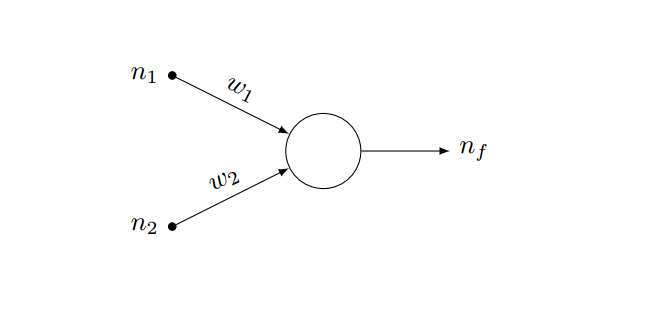
\includegraphics[scale=0.5]{img/rn01.png}
		\caption{La unidad básica de la red neuronal: el perceptrón. Entradas $n_1$ y $n_2$ con peso $w_1$ y $w_2$ respectivamente. 
		La salida $n_f$ es 0 ó 1.}
	\end{figure}
\end{frame}

\begin{frame}{Ejemplo}
	\begin{itemize}
		\item ¿Cómo usamos una red neuronal para saber cuánto vale cada examen?\pause 
		\item Aquí nos bastará con la unidad fundamental de la red neuronal: \textbf{el perceptrón}.\pause  
		\item Un perceptrón es un elemento que tiene varias entradas con un cierto peso cada una.\pause  
		\item Si la suma de esas entradas por cada peso es mayor que un determinado número, la salida del perceptrón es un uno.\pause 
		\item Si es menor, la salida es un cero.
	\end{itemize}
\end{frame}

\begin{frame}{Ejemplo}
	\begin{itemize}
		\item En el ejemplo, las entradas serían las dos notas de los exámenes. \pause 
		\item Si la salida es uno (esto es, la suma de las notas por su peso correspondiente es mayor que cinco), es un aprobado. \pause
		\item Si es cero, no aprobado. 
	\end{itemize}
	\begin{align*}
		n_1w_1 + n_2w_2 \geq 6  \Rightarrow  n_f=1 \\
		n_1w_1 + n_2w_2 < 6  \Rightarrow n_f=0 
	\end{align*}
\end{frame}

\begin{frame}{Ejemplo}
	\begin{itemize}
		\item Los pesos $w_1$ y $w_2$ son lo que tenemos que encontrar con el entrenamiento.\pause
		\item El entrenamiento consistirá en empezar con dos pesos aleatorios ($w_1+w_2=1$) y ver qué resultado da la red neuronal para cada alumno.\pause
		\item También se podría comenzar con puede ser también comenzar con $w_1=w_2=0.5$.\pause 
		\item Si falla en algún caso, se debe ajustar los pesos gradualmente hasta que se obtenga el resultado esperado.\pause
		\item La idea del ajuste o retroalimentación es adaptar la red a la información \textit{oculta} que tienen los datos (interpretación) 
			para que la neurona aprenda.
	\end{itemize}
\end{frame}

\begin{frame}{Ejemplo}
	\begin{itemize}
		\item Si ahora fueran tres exámenes se necesitarían tres nodos de entrada\pause
		\item Si se desean más resultados, se pueden tener tantos perceptrones como salidas se requieran\pause
	\end{itemize}
	\begin{figure}
		\centering
		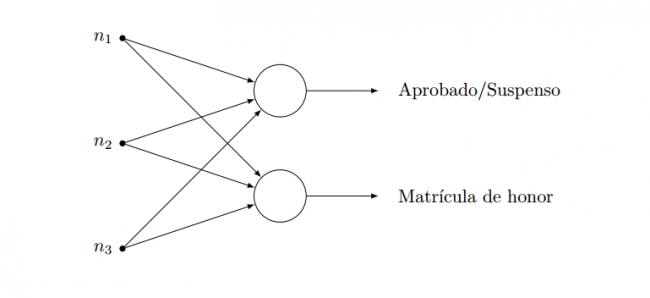
\includegraphics[scale=0.65]{img/rn02.png}
	\end{figure}
\end{frame}

\begin{frame}{Ejemplo - Redes multicapa}
	\begin{itemize}
		\item Suponga ahora que dos alumnos tienen la misma nota en los exámenes, dos dieces.\pause
		\item Uno de los alumnos tiene un 7 en un trabajo y el otro alumno tiene 4.\pause
		\item El primer estudiante aprobó el curso y el segundo no lo aprobó.\pause
		\item Otro alumno tiene un 10 en el trabajo y 4.99 en los dos exámenes y no aprobó.
	\end{itemize}
\end{frame}

\begin{frame}{Ejemplo - Redes multicapa}
	\begin{itemize}
		\item Se puede entrenar una red neuronal con los datos anteriores\pause
		\item Para que la red funcione bien se necesita otro perceptrón intermedio que determine si el 
		trabajo fue aprobado o no aprobado.\pause
	\end{itemize}
	\begin{figure}
		\centering
		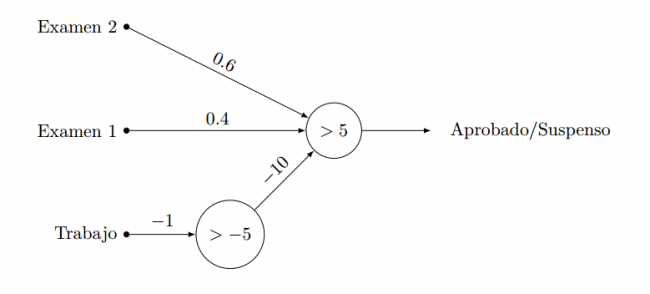
\includegraphics[scale=0.6]{img/rn03.png}
	\end{figure}
\end{frame}

\begin{frame}{Ejemplo - Redes multicapa}
	\begin{itemize}
		\item El primer perceptrón determina si la nota multiplicada por $-1$ es mayor que cinco (esto es, si
			la nota es mayor que 5).\pause
		\item Si así lo es, entonces la salida del perceptrón es 1.\pause
		\item Esta es una red neuronal con dos perceptrones y dos capas.\pause
		\item Lo que se ha logrado con las dos capas es añadir información que no estaba antes.\pause
		\item Lo que se suele hacer es poner varias con varios nodos, cada uno conectado a todas las entradas anteriores.\pause
		\item Durante el proceso de aprendizaje, cada capa \textit{aprende} a encontrar y detectar las características 
			que mejor ayudan a clasificar los datos.
	\end{itemize}
\end{frame}

\begin{frame}{Ejemplo - Sigmoide}
	\begin{itemize}
		\item Si las condiciones en la red neuronal se complican, es posible que los perceptrones ya no sean 
			suficientes.\pause
		\item Para esos casos se puede usar una función más suave, como la \textbf{sigmoide}.\pause
	\end{itemize}
	\begin{figure}
		\centering
		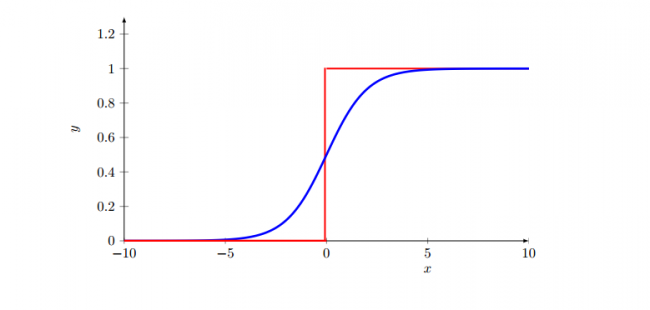
\includegraphics[scale=0.6]{img/rn04.png}
		\caption[short]{En rojo, la función escalón. En azul, la sigmoide, una aproximación más suave.}
	\end{figure}
\end{frame}

\begin{frame}{Redes convolucionales}
	\begin{itemize}
		\item Las redes convolucionales funcionan muy bien en reconocimiento de voz y procesamiento de imágenes. \pause
		\item En una red neuronal se pone una neurona para cada píxel de una imagen\pause 
		\item También se ponen varias capas con varias neuronas, todas conectadas entre sí. \pause
	\end{itemize}
	\begin{figure}
		\centering
		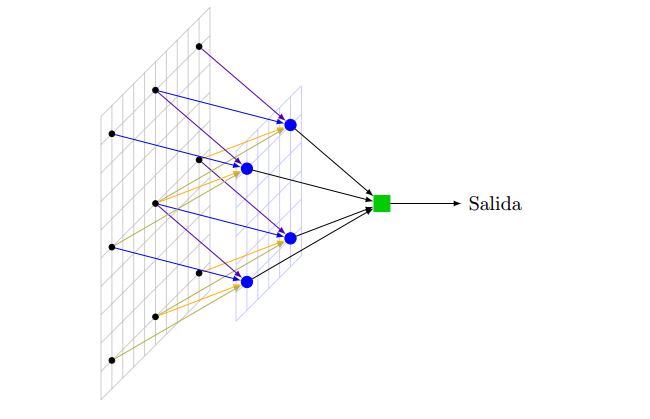
\includegraphics[scale=0.5]{img/rn05.png}
	\end{figure}
\end{frame}

\begin{frame}{Redes convolucionales}
	\begin{itemize}
		\item La idea de las redes convolucionales es tratar de buscar características locales en pequeños 
			grupos de entradas\pause
		\item Se utiliza un mismo grupo de neuronas por cada grupo de entradas \pause
		\item Por ejemplo, un cuadrado de 3x3 píxeles en una imagen o una secuencia de 4 mediciones en un 
			archivo de sonido \pause
		\item Todos los elementos en la capa, llamada \textbf{capa de convolución}, tienen los mismos pesos 
			por cada entrada.\pause
		\item Mientras más capas hayan, la red neuronal podrá descubrir más y más complejas características 
			de la imagen.
	\end{itemize}
\end{frame}

\section{Entrenamiento de una RN}
\begin{frame}{Entrenamiento de una Red Neuronal}
	\begin{itemize}
		\item El proceso de entrenamiento de una red neuronal implica presentar ejemplos de entrenamiento a la red, comparar las salidas 
			predichas con las salidas deseadas y ajustar los pesos de las conexiones para minimizar la diferencia entre ellas.\pause
		\item Esto se logra mediante algoritmos de optimización, como el descenso del gradiente, que ajustan gradualmente los pesos 
			para mejorar el rendimiento de la red en la tarea específica.\pause
		\item El entrenamiento de redes neuronales es el proceso de enseñar a una red neuronal a realizar una tarea.\pause 
		\item En principio, las redes neuronales aprenden procesando varios conjuntos grandes de datos etiquetados o sin etiquetar.\pause
		\item Debido a que utilizan estos ejemplos, pueden procesar entradas desconocidas con mayor precisión.
	\end{itemize}
\end{frame}

\begin{frame}{Entrenamiento de una Red Neuronal}
	\begin{itemize}
		\item Las redes neuronales son capaces de aprender a partir de datos y generalizar a nuevas situaciones\pause 
		\item Esto las hace adecuadas para una amplia gama de aplicaciones en Machine Learning, como:\pause
			\begin{itemize}
				\item Reconocimiento de imágenes \pause
				\item Procesamiento del lenguaje natural\pause
				\item Detección de fraudes\pause
				\item Predicción de series temporales \pause
				\item entre otras. \pause
			\end{itemize}
		\item Su capacidad para capturar patrones complejos y realizar tareas de manera no lineal las ha convertido en una herramienta 
		poderosa en el campo del aprendizaje automático.
	\end{itemize}
\end{frame}

\section{¿Para que sirven las RN?}
\begin{frame}{¿Para que sirven las RN?}
	Las redes neuronales están presentes en varios casos de uso en muchos sectores, como los siguientes:\pause
	\begin{itemize}
		\item Diagnóstico médico mediante la clasificación de imágenes médicas \pause
		\item Marketing orientado mediante el filtrado de redes sociales y el análisis de datos de comportamiento\pause
		\item Predicciones financieras mediante el procesamiento de datos históricos de instrumentos financieros\pause
		\item Previsión de la carga eléctrica y la demanda de energía\pause 
		\item Proceso y control de calidad\pause 
		\item Identificación de compuestos químicos
	\end{itemize}
\end{frame}

\begin{frame}{¿Para que sirven las RN?}
	Cuatro de las aplicaciones más importantes de las redes neuronales son: \pause
	\begin{itemize}
		\item Visión artificial \pause
		\item Reconocimiento de voz\pause
		\item Procesamiento de lenguaje natural\pause
		\item Motores de recomendaciones
	\end{itemize}
\end{frame}

\begin{frame}{Visión artificial}
	La visión artificial es la capacidad que tienen las computadoras para extraer información y conocimientos de imágenes y videos.\pause 
	Con las redes neuronales, las computadoras pueden distinguir y reconocer imágenes de forma similar a los humanos.\pause
	La visión artificial tiene varias aplicaciones, como las siguientes:\pause
	\begin{itemize}
		\item Reconocimiento visual en los vehículos autónomos para que puedan reconocer las señales de tráfico y a otros usuarios del camino \pause
		\item Moderación de contenido para eliminar de forma automática los contenidos inseguros o inapropiados de los archivos de imágenes y videos\pause
		\item Reconocimiento facial para identificar rostros y reconocer atributos como ojos abiertos, gafas y vello facial\pause
		\item Etiquetado de imágenes para identificar logotipos de marcas, ropa, equipos de seguridad y otros detalles de la imagen
	\end{itemize}
\end{frame}

\begin{frame}{Reconocimiento de voz}
	Las redes neuronales pueden analizar el habla humana a pesar de los diferentes patrones de habla, el tono, el idioma y el acento.\pause
	Los asistentes virtuales como Amazon Alexa y el software de transcripción automática utilizan el reconocimiento de voz para realizar
	tareas como las siguientes:\pause
	\begin{itemize}
		\item Asistir a los agentes de los centros de llamadas y clasificar las llamadas de forma automática\pause
		\item Convertir las conversaciones clínicas en documentación en tiempo real\pause
		\item Subtitular con precisión videos y grabaciones de reuniones para aumentar el alcance del contenido	
	\end{itemize}
\end{frame}

\begin{frame}{Procesamiento de lenguaje natural}
	El procesamiento de lenguaje natural (PLN) es la capacidad de procesar texto natural creado por humanos.\pause
	Las redes neuronales ayudan a las computadoras a obtener información y significado a partir de los datos y los documentos de texto.\pause
	El PLN está presente en varios casos de uso, entre los que se incluyen los siguientes:\pause
	\begin{itemize}
		\item Chatbots y agentes virtuales automatizados \pause
		\item Organización y clasificación automáticas de datos escritos\pause 
		\item Análisis de inteligencia empresarial de documentos con formato largo, como emails y formularios\pause 
		\item Indexación de frases clave que indican sentimientos, como los comentarios positivos y negativos en las redes sociales\pause
		\item Resumen de documentos y producción de artículos para un tema determinado
	\end{itemize}
\end{frame}

\begin{frame}{Motores de recomendaciones}
	\begin{itemize}
		\item Las redes neuronales pueden hacer un seguimiento de la actividad del usuario para elaborar recomendaciones personalizadas.\pause
		\item También pueden analizar todo el comportamiento de los usuarios y descubrir productos o servicios nuevos que interesen a un 
			usuario específico.\pause
		\item Por ejemplo, Curalate, una empresa emergente con sede en Filadelfia, ayuda a las marcas a convertir las publicaciones en las 
			redes sociales en ventas.\pause 
		\item Las marcas utilizan el servicio de etiquetado inteligente de productos (IPT) de Curalate para automatizar la recopilación y 
			la selección del contenido social que generan los usuarios.\pause
		\item El IPT utiliza las redes neuronales para encontrar y recomendar de forma automática productos relevantes para la actividad 
			del usuario en las redes sociales.\pause 
		\item Los consumidores no tienen que buscar en los catálogos en línea para encontrar un producto específico a partir de una imagen 
			en las redes sociales.\pause  
		\item En cambio, pueden utilizar el etiquetado automático de productos de Curalate para comprar el producto con facilidad.
	\end{itemize}
\end{frame}

\section{Tipos de RN}
\begin{frame}{Tipos de Redes Neuronales}
	\begin{itemize}
		\item Las redes neuronales pueden tener diferentes arquitecturas, pero una de las más comunes es la red neuronal multicapa o 
			feedforward.\pause 
		\item Esta red consta de una capa de entrada, una o varias capas ocultas y una capa de salida.\pause
		\item La información fluye desde la capa de entrada a través de las capas ocultas hasta la capa de salida, sin retroalimentación.
	\end{itemize}
\end{frame}

\begin{frame}{Ejemplos de algunos tipos de RN}
	\textbf{Redes neuronales prealimentadas}
	\begin{itemize}
		\item Las redes neuronales prealimentadas procesan los datos en una dirección, desde el nodo de entrada hasta el nodo de salida. \pause
		\item Todos los nodos de una capa están conectados a todos los nodos de la capa siguiente.\pause
		\item Una red prealimentada utiliza un proceso de retroalimentación para mejorar las predicciones a lo largo del tiempo.
	\end{itemize}
\end{frame}

\begin{frame}{Ejemplos de algunos tipos de RN}
	\begin{description}
		\item[Algoritmo de retropropagación] Las redes neuronales artificiales aprenden de forma continua mediante el uso de bucles de 
			retroalimentación correctivos para mejorar su análisis predictivo.\pause En pocas palabras, puede pensar en los datos que 
			fluyen desde el nodo de entrada hasta el nodo de salida a través de muchos caminos diferentes en la red neuronal. \pause 
			Solo un camino es el correcto: el que asigna el nodo de entrada al nodo de salida correcto.\pause  
			Para encontrar este camino, la red neuronal utiliza un bucle de retroalimentación que funciona de la siguiente manera:\pause
	\end{description}
	\begin{enumerate}
		\item Cada nodo intenta adivinar el siguiente nodo de la ruta. \pause
		\item Se comprueba si la suposición es correcta. Los nodos asignan valores de peso más altos a las rutas que conducen a más 
			suposiciones correctas y valores de peso más bajos a las rutas de los nodos que conducen a suposiciones incorrectas.\pause
		\item Para el siguiente punto de datos, los nodos realizan una predicción nueva con las trayectorias de mayor peso y 
			luego repiten el paso 1.	
	\end{enumerate}
\end{frame}

\begin{frame}{Ejemplos de algunos tipos de RN}
	\textbf{Redes neuronales convolucionales}\pause
	\begin{itemize}
		\item Las capas ocultas de las redes neuronales convolucionales realizan funciones matemáticas específicas, 
			como la síntesis o el filtrado, denominadas convoluciones.\pause
		\item Son muy útiles para la clasificación de imágenes porque pueden extraer características relevantes de 
			las imágenes que son útiles para el reconocimiento y la clasificación de imágenes. \pause
		\item La forma nueva es más fácil de procesar sin perder características que son fundamentales para hacer 
			una buena predicción.\pause 
		\item Cada capa oculta extrae y procesa diferentes características de la imagen, como los bordes, el color 
			y la profundidad.
	\end{itemize}
\end{frame}

\section{Arquitectura de las RN}
\begin{frame}{Arquitectura de las RN}
	\begin{itemize}
		\item El cerebro humano es lo que inspira la arquitectura de las redes neuronales. \pause
		\item Las células del cerebro humano, llamadas neuronas, forman una red compleja y con un alto nivel de interconexión 
			y se envían señales eléctricas entre sí para ayudar a los humanos a procesar la información. \pause
		\item De manera similar, una red neuronal artificial está formada por neuronas artificiales que trabajan 
			juntas para resolver un problema.\pause 
		\item Las neuronas artificiales son módulos de software, llamados nodos, y las redes neuronales artificiales son 
			programas de software o algoritmos que, en esencia, utilizan sistemas informáticos para resolver cálculos matemáticos.
	\end{itemize}
\end{frame}

\begin{frame}{Arquitectura de una red neuronal simple}
	\textbf{Arquitectura de una red neuronal simple}\\
	Una red neuronal básica tiene neuronas artificiales interconectadas en tres capas:
	\begin{description}
		\item[Capa de entrada.] La información del mundo exterior entra en la red neuronal artificial desde la 
			capa de entrada.\pause Los nodos de entrada procesan los datos, los analizan o los clasifican y los pasan 
			a la siguiente capa.
		\item[Capa oculta. ] Las capas ocultas toman su entrada de la capa de entrada o de otras capas ocultas. \pause
			Las redes neuronales artificiales pueden tener una gran cantidad de capas ocultas.\pause Cada capa oculta 
			analiza la salida de la capa anterior, la procesa aún más y la pasa a la siguiente capa.\pause
		\item[Capa de salida. ] La capa de salida proporciona el resultado final de todo el procesamiento de datos 
			que realiza la red neuronal artificial.\pause Puede tener uno o varios nodos.\pause Por ejemplo, si tenemos 
			un problema de clasificación binaria (sí/no), la capa de salida tendrá un nodo de salida que dará como 
			resultado 1 o 0.\pause Sin embargo, si tenemos un problema de clasificación multiclase, la capa de salida 
			puede estar formada por más de un nodo de salida.
	\end{description}
\end{frame}

\begin{frame}{Arquitectura de una red neuronal profunda}
	\textbf{Arquitectura de una red neuronal profunda}
	\begin{itemize}
		\item Las redes neuronales profundas, o redes de aprendizaje profundo, tienen varias capas ocultas con millones 
			de neuronas artificiales conectadas entre sí.\pause
		\item Un número, denominado peso, representa las conexiones entre un nodo y otro.\pause 
		\item El peso es un número positivo si un nodo estimula a otro, o negativo si un nodo suprime a otro.\pause 
		\item Los nodos con valores de peso más altos tienen mayor influencia en los demás nodos.\pause
		\item En teoría, las redes neuronales profundas pueden asignar cualquier tipo de entrada a cualquier tipo de salida. \pause
		\item Sin embargo, también necesitan mucho más entrenamiento en comparación con otros métodos de machine learning. \pause
		\item Necesitan millones de ejemplos de datos de entrenamiento en lugar de los cientos o miles que podría necesitar una 
			red más simple.
	\end{itemize}
\end{frame}

\section{Comparación entre ML y DL}
\begin{frame}{Comparación entre machine learning y aprendizaje profundo}
	\begin{itemize}
		\item La inteligencia artificial es el campo de las ciencias de la computación que investiga métodos para dar a las 
			máquinas la capacidad de realizar tareas que requieren inteligencia humana.\pause 
		\item El machine learning es una técnica de inteligencia artificial que otorga a las computadoras acceso a conjuntos 
			de datos muy grandes y les enseña a aprender de estos datos.\pause
		\item El software de machine learning encuentra patrones en los datos existentes y los aplica a datos nuevos para 
			tomar decisiones inteligentes. \pause 
		\item El aprendizaje profundo es un subconjunto del machine learning que utiliza las redes de aprendizaje profundo 
			para procesar los datos.
	\end{itemize}
\end{frame}

\begin{frame}{Comparación entre machine learning y aprendizaje profundo}
	\begin{itemize}
		\item Los métodos tradicionales de ML requieren la intervención humana para que el software de machine learning 
			funcione suficientemente bien.\pause 
		\item Un científico de datos determina de forma manual el conjunto de características relevantes que el software 
			debe analizar.\pause 
		\item Esto limita la capacidad del software, lo que hace que su creación y administración sean tediosas.
	\end{itemize}
\end{frame}

\begin{frame}{Comparación entre machine learning y aprendizaje profundo}
	\begin{itemize}
		\item Por otro lado, en el aprendizaje profundo, el científico de datos solo proporciona datos sin procesar al 
			software.\pause 
		\item La red de aprendizaje profundo obtiene las características por sí misma y aprende de forma más independiente.\pause
		\item Puede analizar conjuntos de datos no estructurados como documentos de texto, identificar qué atributos de los 
			datos deben priorizarse y resolver problemas más complejos.
	\end{itemize}
\end{frame}

\begin{frame}{Comparación entre machine learning y aprendizaje profundo}
	Por ejemplo, si se entrenara un software de machine learning para identificar la imagen de una mascota de forma correcta, 
	debería seguir estos pasos:\pause

	\begin{itemize}
		\item Encontrar y etiquetar de forma manual miles de imágenes de mascotas, como gatos, perros, caballos, hámsters, loros, etc.\pause
		\item Indicar al software de machine learning qué características debe buscar para poder identificar la imagen mediante la eliminación. 
			Por ejemplo, podría contar el número de patas, comprobar la forma de los ojos, la forma de las orejas, la cola, el pelo, etc.
	\end{itemize}	
\end{frame}

\begin{frame}{Comparación entre machine learning y aprendizaje profundo}
	\begin{itemize}
		\item Evaluar y cambiar de forma manual los conjuntos de datos etiquetados para mejorar la precisión del software. 
			Por ejemplo, si su conjunto de entrenamiento cuenta con demasiadas fotos de gatos negros, el software identificará de forma 
			correcta a un gato negro pero no a uno blanco.\pause
		\item En el aprendizaje profundo, sin embargo, las redes neuronales procesarían todas las imágenes y determinarían de forma automática 
			que necesitan analizar primero el número de patas y la forma de la cara, y mirar las colas en último lugar para identificar con 
			éxito el animal en la imagen.
	\end{itemize}	
\end{frame}


\section{Bibliografía}
\begin{frame}[allowframebreaks]{References}
    \nocite{*}
    \bibliographystyle{plain}
    \bibliography{biblioRN}
\end{frame}


\end{document}
